\documentclass{tufte-handout}

%\geometry{showframe}% for debugging purposes -- displays the margins

\usepackage{amsmath}

% Set up the images/graphics package
\usepackage{graphicx}
\setkeys{Gin}{width=\linewidth,totalheight=\textheight,keepaspectratio}
\graphicspath{{graphics/}}

\title{Adrenals and Stress Hormones}
\author{Dave Bridges, Ph.D.}
%\date{24 January 2009}  % if the \date{} command is left out, the current date will be used

% The following package makes prettier tables.  We're all about the bling!
\usepackage{booktabs}

% The units package provides nice, non-stacked fractions and better spacing
% for units.
\usepackage{units}

% The fancyvrb package lets us customize the formatting of verbatim
% environments.  We use a slightly smaller font.
\usepackage{fancyvrb}
\fvset{fontsize=\normalsize}

% Small sections of multiple columns
\usepackage{multicol}

% Provides paragraphs of dummy text
\usepackage{lipsum}

% These commands are used to pretty-print LaTeX commands
\newcommand{\doccmd}[1]{\texttt{\textbackslash#1}}% command name -- adds backslash automatically
\newcommand{\docopt}[1]{\ensuremath{\langle}\textrm{\textit{#1}}\ensuremath{\rangle}}% optional command argument
\newcommand{\docarg}[1]{\textrm{\textit{#1}}}% (required) command argument
\newenvironment{docspec}{\begin{quote}\noindent}{\end{quote}}% command specification environment
\newcommand{\docenv}[1]{\textsf{#1}}% environment name
\newcommand{\docpkg}[1]{\texttt{#1}}% package name
\newcommand{\doccls}[1]{\texttt{#1}}% document class name
\newcommand{\docclsopt}[1]{\texttt{#1}}% document class option name

\begin{document}

\maketitle% this prints the handout title, author, and date

\begin{abstract}
\noindent This lecture covers the role of the adrenal glands.  The major topics covered will be the regulation of salt balance by aldosterone and stress responses mediated by adrenal gland secretions.  This lecture covers the following pages in the textbook: 169, 321,326, 344-349, 394-5, 514-5 and 583\cite{Widmaier2013}.
\end{abstract}

\tableofcontents

\pagebreak

\section{Learning Objectives}
For this lecture, the learning objectives are:
\begin{itemize}
\item Name three zones in the adrenal cortex and major regulator(s) of each zone.
\item Name three steroidogenesis pathways and their major products.
\item Explain briefly the physiological mechanism of adrenogenital syndrome.
\item Describe the physiological actions and roles of aldosterone.
\item Explain briefly the renin-angiotensin system.
\item Describe the negative feedback regulation of aldosterone and its relationship to blood volume/blood pressure homeostasis.
\item Describe hepatic and extrahepatic metabolic actions of glucocorticoids. Discuss their relationship.
\item State the major findings caused by adrenal hypersecretion of mineralocorticoids.
\item State the major findings caused by adrenal hypersecretion of glucocorticoids.
\item Name the major hormones secreted from the adrenal medulla. Discuss the differences of epinephrine (epi) and norepinephrine (NE) in cardiovascular actions (physiological levels). 
\item List the major metabolic actions of catecholamines.
\item Contrast the thresholds for actions vs. plasma levels of epi and NE under common conditions, like exercise, and in the disease pheochromocytoma

\end{itemize}

\pagebreak

\section{Anatomy of the Adrenal Gland}

The adrenal gland is located above the kidney and releases hormones in response to either nervous or hormonal stimulation.  The central part of the adrenal gland, known as the adrenal medulla releases epinephrine and norepinephrine which are biogenic amines.  The three regions of the adrenal medulla\sidenote{zona glomerulosa, zona fasciculata and zona reticularis} release steroid hormones including aldosterone\sidenote{a mineralcorticoid}, cortisol\sidenote{a glucocorticoid}, and androstenedione (see Figure \ref{fig:adrenal-anatomy}).  These pathways all initiate from cholesterol, but involve activation of different enzymes to generate these chemically similar, but functionally distinct hormones.

\begin{marginfigure}
  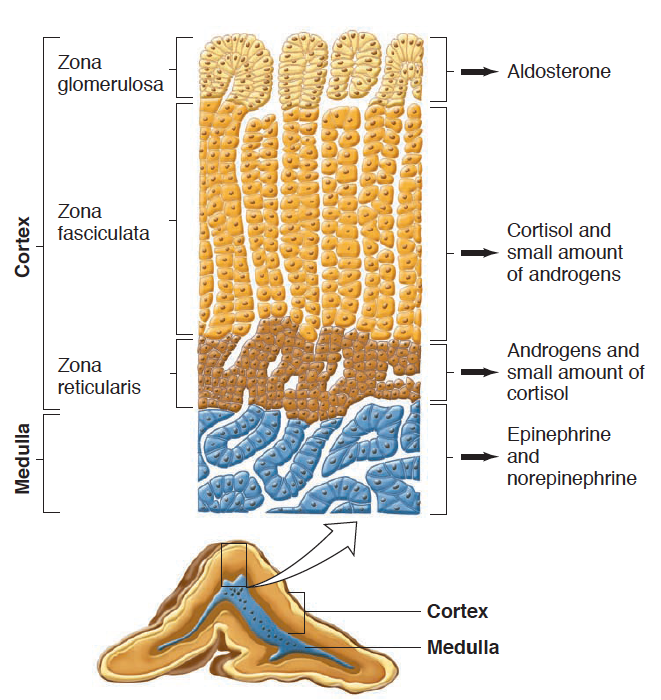
\includegraphics{figures/adrenal-anatomy}
  \caption{The anatomy of the adrenal gland.}
    \label{fig:adrenal-anatomy}
\end{marginfigure}

\section{Steroid Hormones Secreted from The Adrenal Gland}

Steroid hormones are synthesized from cholesterol via enzymes which are regulated by PKA signaling.  In response to the synthetic signal\sidenote{ACTH for cortisol; Angiotensin II for aldosterone}, the GPCR's are activated resulting in cAMP/PKA or IP3 signaling cascades.  Since steroid hormones are membrane soluble they can be released from the cell.  They move through the serum bound to proteins called globulins which keep them soluble in the blood stream.  Both aldosterone and cortisol signal via nuclear receptor signaling mechanisms in their target cells.

\subsection{Aldosterone}

Aldosterone, which is a mineralcorticoid is primarily responsible for sensing and modulating salt balance at the kidney.  It is produced in the adrenal cortex in a region called the zona glomerulosa.  The main site of action of aldosterone is the cortical collecting ducts and the distal convoluted tubule, where it functions to stimulate sodium re-absoroption.  

\newthought{The mineralcorticoid receptor} binds to aldosterone, which then promotes the transcription of three important genes involved in salt reuptake:

\begin{description}
 \item[Sodium/potassium pumps.]  These pumps exchange sodium for potassium, to move sodium out of the kidney and back into the blood.
 \item[ENac] This is a sodium transporter that helps get sodium from the tubule into the cells of the collecting duct.
 \item[SGK1] Is a protein kinase that activates several transporters by post-translational modification.
\end{description}

Together these genes when activated by aldosterone enhance the movement of sodium ions out of the kidney and back into the blood stream.  In the absence of aldosterone, the human body would secrete about 35g of sodium chloride per day.  When aldosterone levels are high (due to reduced sodium concentration), nearly all sodium is reabsorbed.  This complex system requires integration of information about blood volume, blood pressure and sympathetic activity.  This integrated endocrine circuite is known as the renin/angiotensin system

\begin{figure}
\centering
  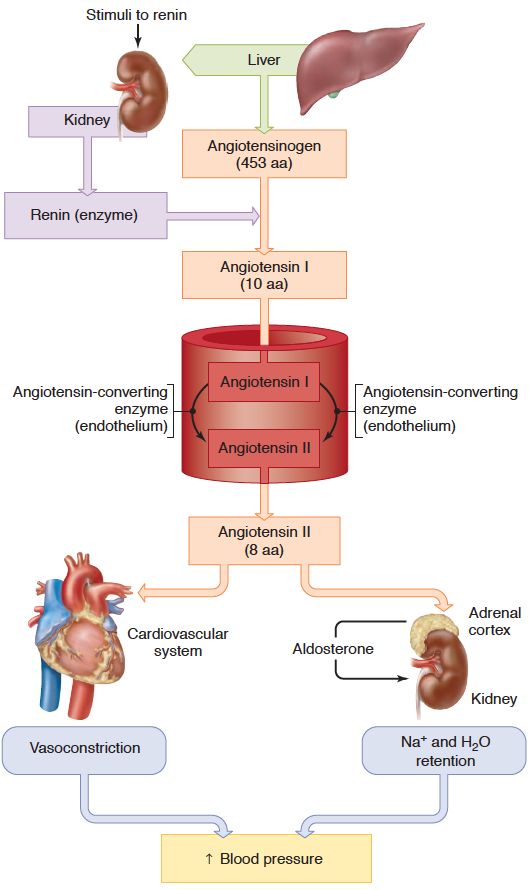
\includegraphics[width=0.5\textwidth]{figures/renin-angiotensin}
  \caption{The renin/angiotensin system.}
    \label{fig:renin-angiotensin}
\end{figure}

\newthought{The Reinin-Angiotensin system.} Angiotensin II\sidenote{the active form} is generated by the liver as a precursor molecule called angiotensinogen.  This molecule is processed in two stages to generate angiotensin II.  The first, and most important regulatory step is mediated by a secreted enzyme known as renin.  Renin is secreted from specialized pericytes near the kidney glomerulus known as juxtaglomerular cells\sidenote{JG cells, see Tigyi lectures for more information}.  When JG cells sense decreased stretch (decreased blood pressure), decreased glomerular flow or have elevated sympathetic nervous activity, Renin is released.  Renin converts angiotensinogen to angiotensin I, which in turn is converted to angiotensin II by angiotensin converting enzyme.  In this way, signaling to JG cells can cause increased angiotensin.  Angiotensin then causes increased vasoconstriction\sidenote{see lectures from O'Connell,  Mancarella and Adebiyi} and increased salt reuptake.  This pathway is illustrated in Figure \ref{fig:renin-angiotensin}.

\subsection{Cortisol}

Cortisol is synthesized and released from the zona fasciculata in response to stimulation by ACTH.  As described previously in the lecture on the anterior pituitary, ACTH is released from the corticotrophic cells of the pituitary in response to the hypothalamic hormone CRH.  Cortisol is elevated under times of psychological stress and is also under the control of a circadian cycle\sidenote{biological process that displays an endogenous, entrainable oscillation of about 24 hours.  For more information see \url{http://en.wikipedia.org/wiki/Circadian_rhythm}}.  Cortisol levels are normally highest in the morning, reaching a peak shortly before waking up and decline during the day.

\newthought{Night shift workers, such as those as the FedEx facility often have altered circadian rhythms and elevated Cortisol levels.}  This predisposes people who have abnormal circadian rhythms to have higher risk of diabetes, cardiovascular disease and sleep disturbances\cite{Scheer2009,Pan2011}.

\newthought{The primary role of cortisol is to maintain blood glucose in times of chronic stress.}  Since most tissues, including the brain require glucose but do not store large amounts of glycogen and lipids they require a stable supply of glucose from the periphery.  Glucose can be released from liver glycogen stores, or produced from precursor molecules\sidenote{amino acids and fatty acids} in the liver via a process known as gluconeogenesis.  Cortisol, through its nuclear hormone receptor the glucocorticoid receptor, activates the transcription of several important gluconeogenic genes in the liver including PEPCK and Pyruvate carboxylase.  To ensure that sufficient precursors are available for hepatic gluconeogenesis, cortisol also activates the breakdown of muscle protein\sidenote{this is known as proteolysis} and adipose triglycerides\sidenote{this is known as lipolysis}.  Finally, cortisol induces resistance to insulin in muscle, adipose and liver tissues.  Normally, insulin functions to pull glucose out of the blood and into muscle and adipose tissue, but cortisol prevents this, in order to maintain glucose levels in the blood.  

\newthought{A second major role of cortisol is to suppress immune function.}  Immune responses are energetically quite costly, so in line with directing nutrients to the brain during stress, immune function is decreased.

\newthought{In addition to its direct effects, cortisol also sensitizes tissues to epinephrine}, so that short-term stress responses can also be activated in times of chronic stress.  This is accomplished by the glucocorticoid receptor directly activating the transcription of the $\beta$-adrenoreceptor gene\cite{Hadcock1988}.

\newthought{Local concentrations of cortisol} are regulated by enzymatic inactivation by an enzyme known as 11$\beta$-hydroxysteroid dehydrogenase 2.  This enzyme serves two important roles.  One is to allow for local (tissue-specific) negative feedback of the cortisol signal.  The other is to prevent tissues that should respond to aldosterone from accidentally responding to elevated levels of the chemically similar cortisol.  By elevating 11$\beta$-hydroxysteroid dehydrogenase 2 activity, cortisol is converted to cortisone which has less affinity for the glucocorticoid receptor.

\newthought{Another negative feedback mechanism for cortisol} is that elevated cortisol levels suppress the release of both CRH (from the hypothalamus) and ACTH (from the anterior pituitary).  This integrated circuit is known as the HPA\sidenote{hypothalamus-pituitary-adrenal} axis.  Cortisol functions at several steps in the immune response, including suppressing both the innate and adaptive immune system.  This is one of the reasons that prednisone\sidenote{a synthetic glucocorticoid} is used as in autoimmune diseases such as asthma, arthritis and allergic disorders.

\section{Epinephrine and Norepinephrine}

In contrast to the steroid hormones described above, the adrenal medulla secretes epinephrine and norepinephrine\sidenote{also known as adrenaline and noradrenaline}, two water soluble biogenic amines\sidenote{also known as catecholamines}.  The adrenal medulla primarily produces epinephrine due to high levels of the enzyme phenylethanolamine-N-methyltransferase.  In contrast to cortisol release, which is in response to stress-induced increases in CRH/ACTH, adrenaline is released after direct sympathetic activation innervation of the adrenal medulla.  This means that adrenaline is increased quickly and results in much more rapid responses than cortisol.  

\newthought{Epinephrine binds to $\alpha$ and $\beta$-adrenergic receptors} which are both GPCRs.  $\beta$-adrenergic receptors are coupled to Gs and their activation results in activation of the cAMP/PKA pathway to mediate most of its cellular effects.  $\alpha$-adrenergic receptors are coupled to Gi, which inhibit PKA signaling or Gq proteins which activate IP3/Ca\textsuperscript{2+} signaling.

\subsection{The Role of Biogenic Amines in Cardiovascular Function}

One major effect of catecholamine release is to increase blood flow to the muscle, as part of the flight or fight response\sidenote{This was covered in more detail by in the lectures given by Drs Mancarella and O'Connell}.  This is accomplished by causing more heart muscle constriction (via $\beta$-adrenergic receptors linked to Gs) while also causing smooth muscle vasodilation (via $\alpha$-adrenergic receptors linked to Gi).  This is also the basis of using beta-blockers\sidenote{$\beta$-adrenergic receptor antagonists} to reduce blood pressure and manage cardiac arrhythmias. 

\subsection{Metabolic Effects of Epinephrine}

In addition to its cardiovascular effects, much like cortisol, adrenaline functions to make more blood glucose available in times of acute stress.  In contrast to the slower acting cortisol, adrenaline promotes rapid breakdown of glycogen and triglycerides to make their products available for muscle oxidation\sidenote{useful when running away from a bear.}.

\newthought{In the liver, where most of the body's glycogen is stored}, $\beta$-adrenergic receptor activation of PKA results in the activation of glycogen phosphorylase\sidenote{the enzyme that breaks glycogen down} and inhibits glycogen synthase.  PKA also induces gluconeogenesis like cortisol, but while cortisol only  transcriptionally activates gluconeogenic enzymes, PKA phosphorylates an enzyme called PFK-2 to induce gluconeogenesis, while also phosphorylating and activating a transcription factor called CREB, in order to transcriptionally increase the levels of gluconeogenic genes.

\newthought{In muscle tissue}, PKA activation induces glycogenolysis, glycolysis\sidenote{glucose breakdown into ATP} and mitochondrial respiration to generate ATP for muscle contraction.  This is in contrast to the liver, where glycolysis is not activated, but instead the glucose is produced is transferred to the muscle for oxidation.  In adipose tissue, epinephrine results in rapid induction of lipolysis by PKA-mediated phosphorylation of triglyceride breakdown enzymes.  These fatty acids are then also oxidized for energy in muscle tissue.

\section{Pathophysiology Related to Adrenal Hormones}

\newthought{Cushings's syndrome\cite{Cushing1932} is the result of elevated cortisol levels}, either due to a pituitary tumor which constitutively secretes ACTH, or an adrenal tumor which constitutively secretes Cortisol.  The primary phenotypes associated with over-production of cortisol are diabetes (elevated blood glucose), muscle weakness, reduced bone mass, reduced immune function and enhanced subcutaneous fat deposition.  Similar phenotypes can also occur with prolonged glucocorticoid treatment, for example when prescribed these as chemotherapeutic or anti-immune function therapies.

\newthought{Conn's syndrome\cite{Conn1955} is similar to Cushing's syndrome} in that it is due to an adrenal cancer, but in this case it is due to a tumor in the zona glomerulosa.  This results in constant overproduction of aldosterone.  This leads to too much salt retention, leading to high blood pressure, headaches and muscle weakness.  Conn's syndrome can be treated by mineralcorticoid receptor antagonists.

\newthought{Addison's disease\cite{Addison1855}} is due to immune destruction of the adrenal gland, functionally also preventing steroid hormone production.  In this case glucocorticoids and mineralcorticoids cannot be made and therefore patients have excessive salt excretion.  Patients are prone to stress-induced hypoglycemia and low blood pressure, a condition known as an Addisonian crisis.  Since there is no feedback from cortisol to the CRH/ACTH axis, ACTH is hyper-produced in this case.  Elevations of ACTH and linked to elevations in another hormone called melanocyte stimulatory hormone\sidenote{$\alpha$-MSH} as they are both produced from the same transcript.  Elevations in $\alpha$-MSH lead to the characteristic hyperpigmentation associated with Addison's disease. 

\newthought{Congenital Adrenal Hyperplasia\sidenote{also known as adrenogenital syndrome}} results from mutations in the biosynthesis genes involved in the production of steroid hormones.  This prevents the synthesis of mineralcorticoids, glucocorticoids and sex steroids.  Since these mutations occur during development, some of the primary phenotypes are reduced development of repdroductive organs and impaired salt balance.  This is a recessive genetic disorder and can often be treated pharmacologically by providing the missing steroid hormones.

\newthought{Pheochromocytoma is due to an overproduction of norepinephrine.}

Pheochromocytoma are tumors that inappropriately secrete adrenaline or noradrenaline at high levels.  Clinically these patients have elevated heart rate, blood pressure and anxiety and undergo rapid weight loss and elevated blood glucose.  These patients are often treated surgically\sidenote{to remove the tumor} and with beta-blockers.
\listoffigures
\listoftables

\bibliography{library}
\bibliographystyle{plainnat}



\end{document}
